\documentclass[paper=a4,twoside=false,BCOR=0mm,DIV=calc,fontsize=12pt]{scrartcl}

\usepackage[automark,headsepline]{scrpage2}
% \usepackage{xunicode,fontspec,xltxtra}
\usepackage[english]{babel}

\usepackage[T1]{fontenc}
\usepackage[utf8x]{inputenc}

\usepackage{graphicx}
\usepackage{lastpage}
\usepackage{listings}

%Schöne Tabellen
\usepackage{booktabs}

%\usepackage{longtable}

\usepackage{multirow}

% Kein einrücken und Abstand zwischen Absätzen.
\usepackage{parskip}
\setlength{\parindent}{0cm}

% Hyperlinks und url's
\usepackage[hidelinks]{hyperref}



% \usepackage[debug]{libertine}
% \setromanfont[Mapping=tex-text]{Linux Libertine O}
% \setsansfont[Mapping=tex-text]{Linux Biolinum O}
% \setmonofont[Mapping=tex-text]{Liberation Mono}

\pagestyle{scrheadings}

\clearscrheadfoot
\ihead{\headmark}
\ohead{Page\pagemark\ of \pageref{LastPage}}
\ifoot{Business frameworks}
\cfoot{{
\includegraphics[width=1.5cm]{./img/CC3.png}}}
\ofoot{\today}

\renewcommand*{\pnumfont}{
	\normalfont\rmfamily\slshape
}

\KOMAoptions{draft=false}
\KOMAoptions{DIV=last}

\begin{document}

% --- Titelseite --- %
\begin{titlepage}
	\enlargethispage{3cm}
	\begin{raggedright}
	\begin{picture}(0,0)
		\put(-30,14){
\includegraphics[width=7cm]{./img/fhnw-technik-head.pdf}}
	\end{picture}

	\vspace*{6cm}
	{\Huge\bfseries\sf
		MAS-IT\\[1.7ex]
	}
	{\Large\bfseries\sf
		Business frameworks in QC laboratory processes\\[2.2ex]
	}
	{\large\bfseries\sf
		Masterthesis von\\[1.5ex]
		Etienne Rebetez\\[1.5ex]
	}
	\vspace*{1.5cm}
	{\large\bfseries\sf
		FHNW\\[1.5ex]
		Hochschule für Technik\\[1.5ex]
		Studiengang MAS-IT\\[1.5ex]
		Betreuender Dozent:\\[1.5ex]
		Dr. sc. techn. Ronald Tanner\\[1.5ex]
	}
	\vspace*{2cm}
	{\large\bfseries\sf
		Bern, \today\\
	}
	\end{raggedright}
\end{titlepage}

\newpage
% --- Zusammenfassung --- %
\section*{Summary}
Text

% --- Vorwort --- %
\section*{Vorwort}
Text
% --- Inhaltsverzeichnis --- %
\newpage
	\tableofcontents

% --- Einleitung --- %
\newpage
\section{Introduction}
Laboratory processes. What is that all about? A simplified view looks like the following. A sample of a certain substance comes into the QC lab. 
The lab performs then the analysis. All used solutions, instruments and steps have to be documented. That is traditionally done on paper. The result is then transferred to the client that ordered the analysis.

What analysis have to be made etc. is given by the labor information and management system (LIMS) \cite{lims}. The LIMS also says when and what sample has to be analysed.

At this point it is important to emphasize that everything that is not documented is not done from an audit point of view (see GMP \cite{gmp}). Also the standard operating procedure (SOP) has to be followed exactly by the lab technician.
After the analysis it is mostly the case to have a calculation step where certain parameters are calculated to get the final value. The final value is then transferred back into the LIMS database. These are mainly manual steps. These manual steps can lead to errors and are time consuming.
Although the operating of balances, creation of solution or other manual tasks cannot be automated, the data flow and the process can.

This report aims to look at the layer between LIMS and the instruments and the analysis method. In the past few years there has been a ton of programs that aim to solve that problem \cite{}.  Some try to achieve that with an almighty LIMS. But since most LIMS programs date from the 90's the implementation is not easy and you end up having a not maintainable huge monolithic system. There is also the idea of electronic lab notebooks (ELN) \cite{eln}. These ELN where usually conceived for R\&D laboratory. That means more freedom and less strict processes.
Then there is the software for the instruments, that can perform more and more tasks. This looks like a good idea, but there are so many instruments, methods and manufactures that there is just no solution that fits it all. Also it is still the case, that one solution of one manufacturer is in no way compatible to the solution of another manufacturer.

This is report therefore explores what existing tool exists in the business IT world and if they could be used to automate a chemical laboratory.

\section{The laboratory landscape}
The laboratory knows many different analytic methods. They all have different requirements and provide different forms of results. That gives us an extremely heterogeneous landscape. 

First we need to look at the current laboratory work flow, with the given programs. Historically, and still so, the lab uses the LIMS to see what samples have do be done and to type the results back. The LIMS is a height level program that was designed to managed samples.

There is also a second program in use. An Scientific data management system SDMS \cite{sdms} database. This stores Raw data from analysis and provides an API to retrieve and query the data.
To normalize the data and provide an easy review ability of every step, a report, that can be viewed and signed in the SDMS database, is created and printed into the database.
The problem with heterogeneous data and raw data reports is currently overcome with the SDMS database. It is possible to print reports into the database and tag them automatically. As a result the reports printed into that database can be parsed and the data is then available in an electronic form. This currently is in place and works pretty well.
It is however mostly implemented in Excel \cite{excel} applications.

\begin{figure}
    \begin{center}
      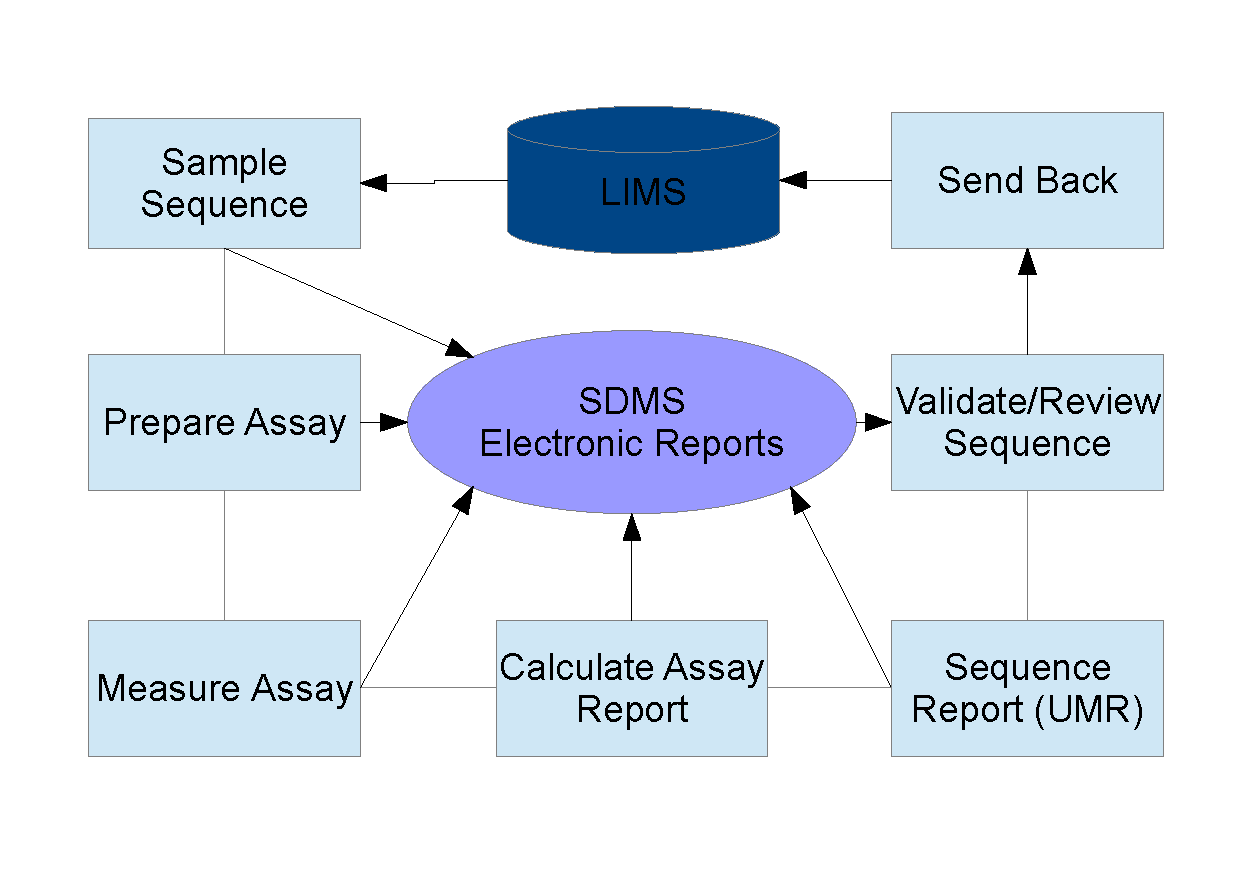
\includegraphics[width=1\textwidth]{./img/Laboverview.pdf}\\
    \end{center}
  \caption{The current lab work flow}
  \label{CurrentLabWorkflow}
\end{figure} 

As you can see in figure \ref{CurrentLabWorkflow} there is a high level process. Each step can have manual user steps or can be done automatically with scripts or some sort of application. 

The assays usually are grouped together in an sequence.

\subsection{Instrument software}
% TODO instrument software exkurs. 


\subsection{Raw data}
The definition of raw data is all the data that a instrument generates. That means the actual measured values. 
This raw data usually needs to be integrated or calculated in some way or another. To be able to check the calculation or just to rerun them the data needs all to be stored in a database. It is also still customary to just store the paper copy.

\section{Concept and Goals}
So the question came up, why not look at something completely different. The lab is not the only business that has processes. There could be other business frameworks that provide the needed functionality. This system should be able to integrate and interface these different islands of programs. It would be like a laboratory middle ware \cite{middleware}. 

To make the automation in such a heterogeneous landscape possible a sort of state machine is needed. This state machine knows how process look like, which processes are currently run, in which state they are in and which is the next to execute.
This pattern is basically the same in every business process. One of the therms is SOA (Service Oriented Architecture) \cite{soa}. The state machine engine would therefore be the heart of the hole automation process.

Since the lab is obviously not the only place in the world that has predefined process a look at generic state machines was imminent.


\subsection{Requirements}
Beside the central process engine, there are also other aspects to be considered. One is a web application that should provide forms and an overview
of the tasks. These human interfaces should also be available on mobile devices.
Since the current implementation is based on Excel sheets, lots of them, it is of importance that the current applications can be implemented and reused in the new framework.
For instance it should be possible to send data to an Excel application and get the results back into the process stream.

\section{Process description languages}
It was decided to use some sort of state machine. To configure these state machine engines there are already several standards. 
Two process definition languages are already well established:

\begin{itemize}
 \item BPEL
 \item BPMN
\end{itemize}

Both are open standards from OMG \cite{omg}.

\subsection{BPEL}
The BPEL (Business Process Execution Language) \cite{bpel} was an answer to the process problem that came from the IT world. It is very technical and the process description is made with ifs and loops that are also known in common programming languages. The definition is made in a XML file. 

\subsection{BPMN}
BPMN (Business Process Model and Notation) \cite{bpmn} has it roots in the business process modelling. It first was only a description language to provide some unified task or gateway definitions. These are the elements of the common flowcharts. 
With the version 2 of the BPMN standard these flowcharts can now be interpreted by an engines and be run as a program.
The definition is made in a XML file. 

The XML configuration describes a process. The process has multiple tasks. These tasks can be another sub process BPMN definition, a program or script that is started via the process engine or a user task that needs an interaction with a human. 

The task of a user is usually to fill out a form (if the data isn't available in the system), start processes or claim tasks to do and review raw data and reports.

\subsection{Process engines}
The engines are implementations of these business description language. The engines provide all sort of logic that would be hard to implement every time from scratch.
\begin{itemize}
  \item What processes are there
  \item Which are in what state
  \item Processes are recoverable and transaction save. (i.e in case of crash)
  \item What happens if a new version of the process is deployed.
  \item Who did what and when. (History and Log service)
\end{itemize}

The last point is important to emphasize. This is a big added value to the existing situation regarding the audit compliance.

\subsection{Engine evaluation}
The business process engine forms the core of the infrastructure. Thus I invested a great amount of time to have a look at different solutions available.

The following chapters present some of these engines that are already available. The list is far from complete and in alphabetical order.

\subsubsection{activeVOS}
activeVOS \cite{activevos} is a product from Active Endpoints, Inc. It uses open standards to implement its feature. The supported notations are BPEL and new also BPMN. Everything is implemented in Java and XML. The editor you get looks and feels like an eclipse plugin. The application runs on an JavaEE application server.

The documentations look good. It has videos, tutorials and they also provide training. 

In addition they have some additional tools to the BPEL engine like reporting.

The cost for the implementations will cost around 50'000 USD \cite{activvosscost}.


\subsubsection{Activiti}
Activiti \cite{activiti} is an open source BPMN engine. It was forked from the jBPM \cite{jbpm} from JBOSS. It is therefore a very young project that has the goal to build a rock solid BPMN engine. Activiti is really only the engine that provide an Java API. There is also a example web application Activiti Explorer that shows and demonstrate the ability of the Activiti engine.

Because it is open source it is free of charge. Although the effort to get a working product might be bigger. 

There is also a company Signavio \cite{signavio} behind Activiti. Signavio provides consulting and BPMN creation tools.

\subsubsection{Apache ODE}
Apache ODE \cite{appacheODE} is an open source BPEL engine. ODE provides an Java API to use in a Java program.
There is also an eclipse plugin, that helps create the BPEL XML definition in a graphical interface.


\subsubsection{ARIS}
ARIS \cite{aris} is a product form software AG. It is a big enterprise BPM solution that brings many tools like process overviews, dashboards, reports or monitoring. ARIS was developed to work well with SAP. Therefore it is by definition an height level implementation.

You buy a solution and the code is not accessible. software AG provides training for employees to configure or work with the product. 

The cost looks to be quit height and is at least 10 Million USD \cite{ariscost}.


\subsubsection{Biztalk}
Biztalk \cite{biztalk} is the BPEL implementation from Microsoft. It is sold as Biztalk server 2010 and is advertised as Business Proces Management (BPM) suite. Since it is a Microsoft product it is written and configured in the .NET programming language. The integration with other Microsoft products like Sharepoint should therefore be good.

The enterprise edition costs around 44'000 USD \cite{biztalkcost}. For testing and development there is a free license.


\subsection{Summary of products}

\begin{center}
\begin{tabular}{l | c c c p{3cm}}
\toprule

Name & Notation & Language & License & Extras \\

\midrule

Activiti & BPMN & Java & Apache 2.0 & only API \\
activVOS & BPMN/BPEL & Java & proprietary &  uses open standars \\
Apache ODE & BPEL & Java & Apache 2.0 &   \\
ARIS & BPMN/BPEL & Java & proprietary &  sold as fully feature product \\
Biztalk & BPEL & .NET & proprietary &  share point integration \\


\bottomrule
\end{tabular}

\label{tab:enginecomparison}
\end{center}

\subsection{Selection}
Since either BPMN nor BPEL is in use at the moment the first thing to decide is what specification to use.
It does not make sense to mix both, unless you already have one in use and wish to use the additional features of the other engine. 

BPMN 2.0 seems to be the better choice due to the close business process view. BPEL exists longer but seems unnecessary complicated.
Therefore BPMN is the better choice for the lab process definition. 

If we now look at the BPMN 2.0 engines, only ActiVOS, Activiti and ARIS remain from the list above.

ActiVOS provides some extra GUI's to give "simpler" access to the configuration. It creates XML and configurations in the background.
They can fortunately be seen and changed from hand. In the bottom line, it seems nice but does not provide a big advantage. Also most documentations is for the BPEL engine.

ARIS is the big all inclusive package. It is however impossible to work yourselves on the project because they sell also the programming and support. Therefore there is no code ore XML visible in the hole package. So for each change the external company has to be contracted.
They provide some basic training courses for configuration.

Activiti has a total other approach. It has no gui what so ever. I provides an open programming interface that provides all functionality 
of the engine. The XML can be easily edited directly. It is therefore slim and sticks to the one task it tries to solve.
The downside is that there is a steep learning curve since everything has to bee implemented in the code. 
Because it is open source there are already some example web application that can be used out of the box. 

\subsection{Conclusion}
The monolithic concept of big systems has proven in the past to be inflexible and heavy on the maintenance. 

The decision was made to use Activiti because of its simplicity and possibility to add other functions (i.e monitoring or reporting) in the future over other programs that also have just one functionality.
Activiti plays also well together with Java based web frameworks like Vaadin \cite{Vaadin}.

% TODO add some Requirement <-> Is comparaison

\subsection{Compatibility}
Although BPMN 2.0 is a standard and provides most keywords and rules the implementations still adds own keywords or extra functionality (i.e forms). So the BPMN files can't just be copied form one engine to another. If you chose one engine it is kind of final and you will have to stick to it.

If an engine change really has to be made it is however simpler to achieve than if you had the complete logic inside the code. If the new engines even
uses the same programming language, it is very probable, that you can just reuse the business logic classes. 


\section{Software Architecture}
The environment consists of an user interface, the BPMN engine, the processes (laboratory methods) and universal usable components (jar archives). Most of the code is written in Java. 

To use the existing Excel applications, a so called calculation server was written. This is a stand alone application and communicates over sockets with the client.

The BPMN process and forms are put together into an own jar archive. These process definitions can be add as dependency to the main application with the BPMN engine.


\begin{figure}
    \begin{center}
      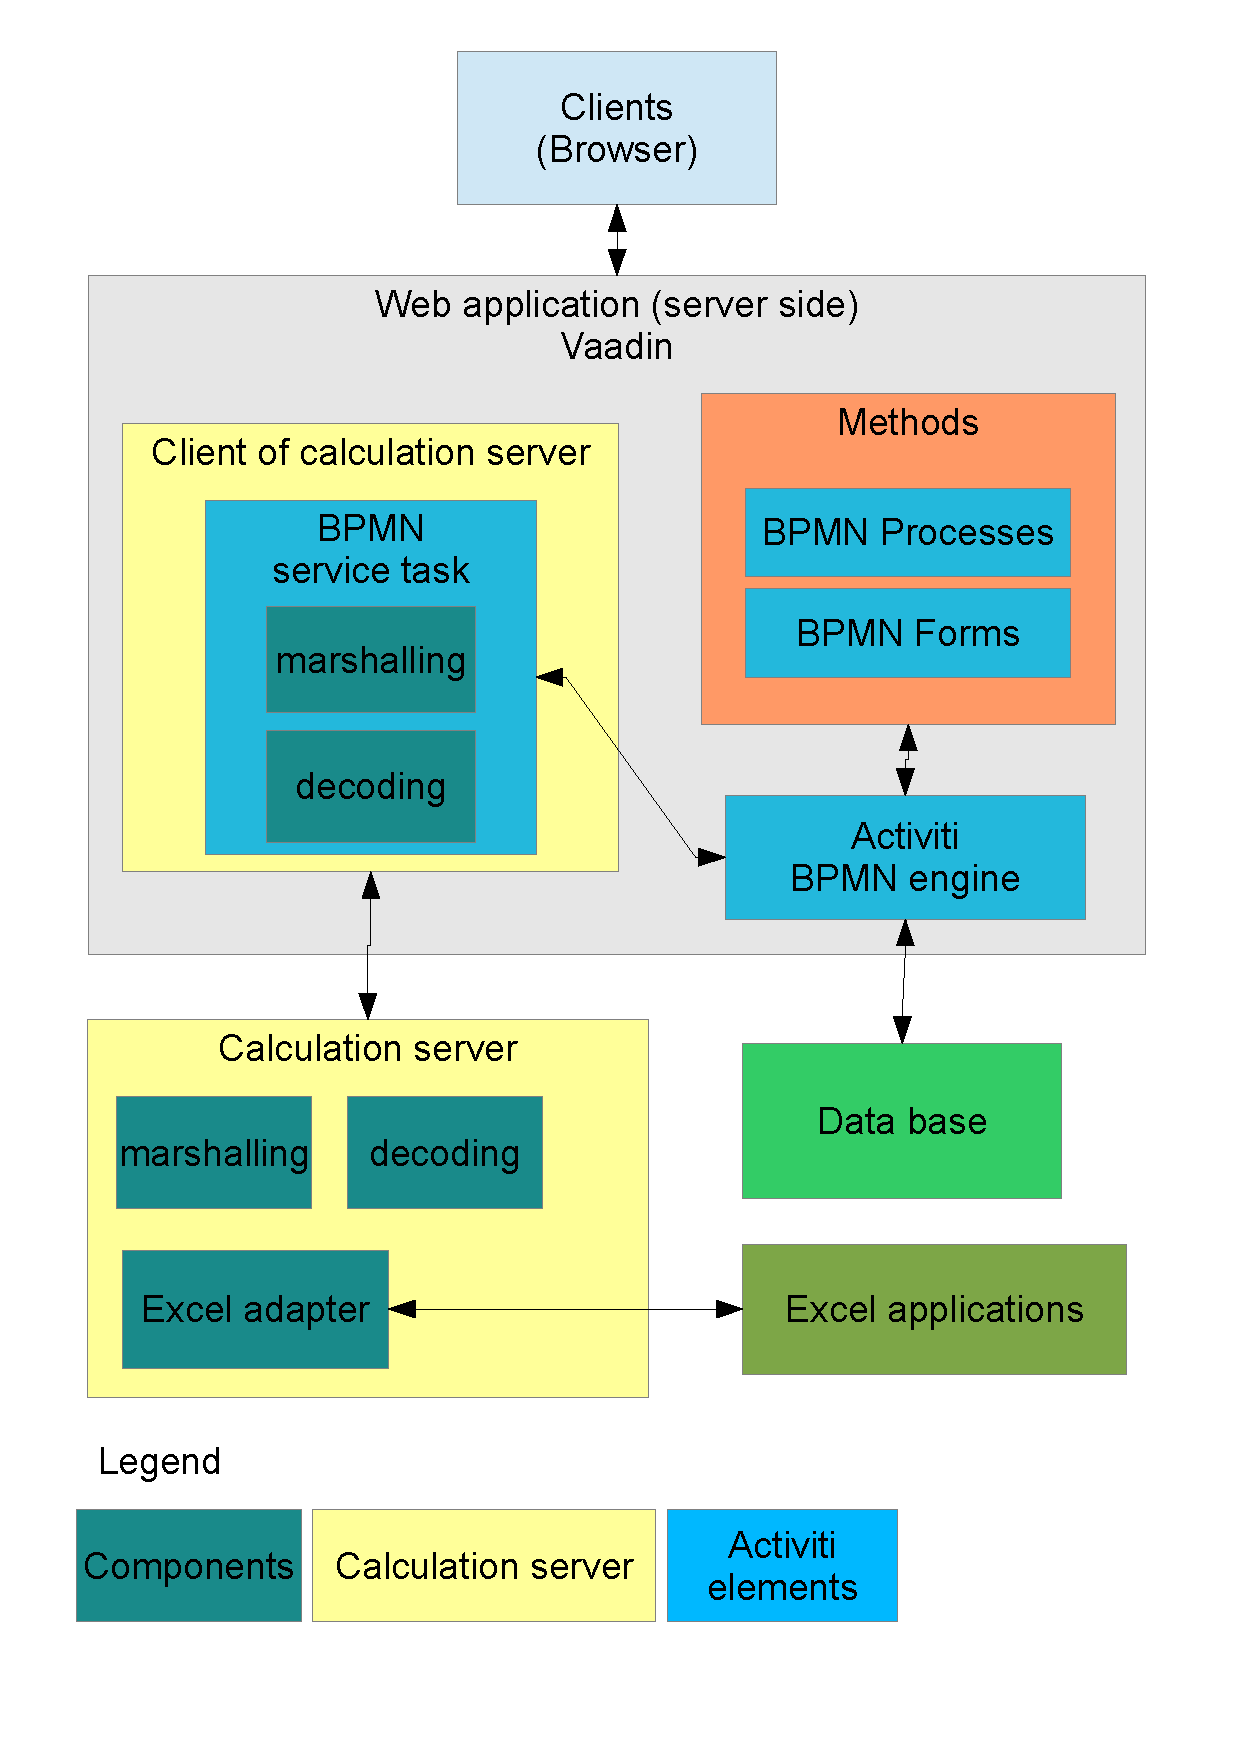
\includegraphics[width=0.8\textwidth]{./img/ArchitectrueOverview.pdf}\\
    \end{center}
  \caption{Overview of the architecture}
  \label{architectureoverview}
\end{figure} 

\subsection{Graphical user interface}
For the graphical user interface (GUI) the web application seems to be a good choice. The web application can be displayed on most devices. With the power of CSS \cite{css} they can even be shown differently on small screens.

To keep things in Java and not being forced to be bothered with the web technology, Vaadin \cite{Vaadin} is used as a web framework.


\subsection{Process engine}
For the process engine Activiti is used. Activiti comes with a variety of services that provides the programmer with methods and informations.

The following services are available \cite{activitijavadoc}:
\begin{itemize}
 \item RuntimeService: Service which provides access to Deployments, ProcessDefinitions and ProcessInstances. 
 \item RepositoryService: Service providing access to the repository of process definitions and deployments. 
 \item TaskService: Service which provides access to Task and form related operations. 
 \item ManagementService: Service for admin and maintenance operations on the process engine. 
 \item IdentityService: Service to manage Users and Groups. 
 \item HistoryService: Service exposing information about ongoing and past process instances. 
 \item FormService: Access to form data and rendered forms for starting new process instances and completing tasks
\end{itemize}

For process related data the runtime service, task service and form service are the mostly used.


\subsection{Configuring}
The Main Application (Web application) is configured using the spring framework \cite{spring}. The Spring framework uses the paradigm of the dependency injection \cite{dependencyInection}.

This allow to configure external components, the database or process parameters in a XML configuration file. The Java code does not have to be modified. 

This way components can be reused in different applications. It is also easy to configure them in unit tests.

\subsection{Dependencies}
Dependencies are provided as own or third party Jar archives that can be added to a JAVA project.
Dependencies can be handled by hand. This is strongly discouraged. In the long run it is way simpler to use build tools that do the dependencies resolvability for you.

When dependencies are defined during the development they should be handled with the following rules to keep it simple:
\begin{itemize}
 \item Components are in the lowest level followed by methods (processes) and then the web applications.
 \item Components do not have dependencies of other components or higher applications like the web application. Only third party packages are allowed.
 \item Methods should only have components and third party packages as dependencies
 \item The web applications should where possible use the components or methods as dependencies. Third party packages are of course also allowed.
\end{itemize}

\section{Example Application}
Now that we have chosen a BPMN process engine and the other required frameworks we need to have a concrete task to try the business framework on. That is why an example application was designed.

The process takes an annual inventory item review. These items are reference samples of the substance that were sold.

\begin{figure}
    \begin{center}
      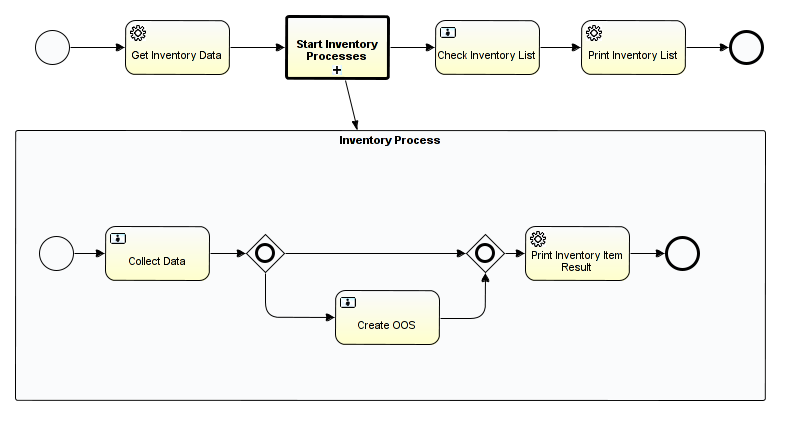
\includegraphics[width=1\textwidth]{./img/PanExampleBPMN.png}\\
    \end{center}
  \caption{Example Application work flow}
  \label{panexampleWorkflow}
\end{figure} 

First a list of the reference samples that have to be checked is retrieved from the parent system (i.e LIMS). This is done with a SQL query on the database. 
The sample number and the location is then stored in a process variable as a data object list.

For each item in the list a sub process is started in parallel (callActiviy). The sub process is a separate BPMN process definition.
The data object which represents a sample, is given to the newly created process.

Now the user can claim the tasks or in this case the samples they wish to check. Then they go to the location and provide the verdict of that sample and a value. If the sample is fine a report is created otherwise a OOS (Out of specification) procedure has to be started first. The OOS process is not part of this demonstration application. It would however be very easy create and to call another sub activity in the future.
To print the reports the existing infrastructure is used. The reports are stored in the SDMS and can be signed there.
Once all samples have been controlled, the parent process goes to the next task.

The laboratory supervisor now gets the task to check the sample list. An overview of the sample list and the verdicts is presented to him. The entered values also gets calculated together. The calculation step is purely for the sake of demonstrations.
The list with all samples is then again printed to the SDMS. That concludes the review process.

This process is used to illustrate the further examples and references.



\section{Web application}

\begin{figure}
    \begin{center}
      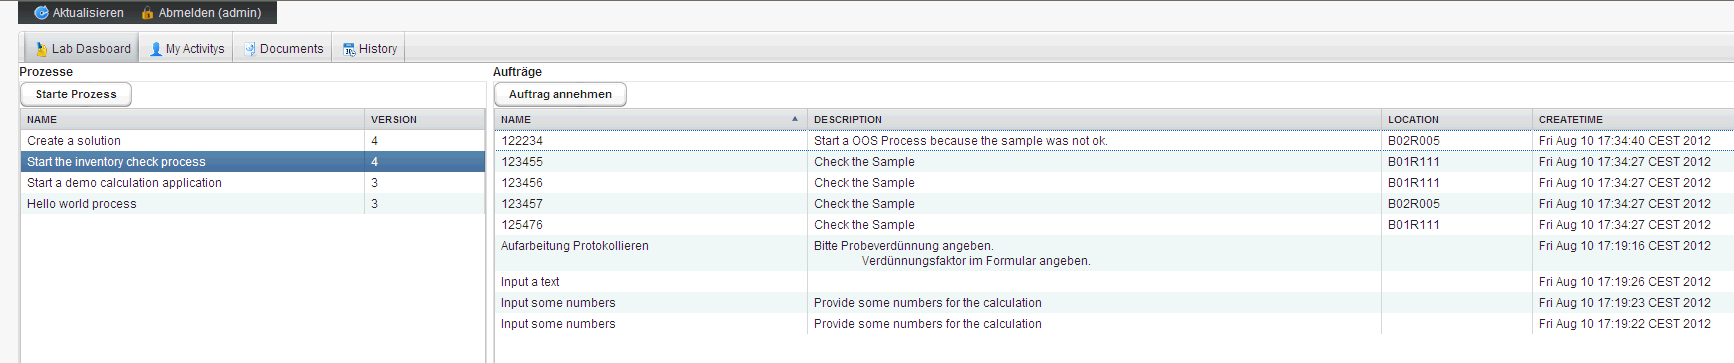
\includegraphics[width=1\textwidth]{./img/LaraWebApplicationScreenshot.png}\\
    \end{center}
  \caption{LaraWebApplication screenshot}
  \label{webapplicationscreenshot}
\end{figure} 

The web application was named LaraWebApplication.

Besides the BPMN engine, the web application is a central cornerstone of this project. After all, that is what the user gets to see.
The decisions was made to use Vaadin \cite{Vaadin} as a web framework. It allows to program the web application completely in Java on the server side. The Java code then gets compiled into (Google web toolkit) GWT \cite{gwt} code. GWT in turn uses HTML5 and Javascipt. So there is
no need to get in trouble with web technology. The HTML is generated for you.

As the back end Activiti is used. So the user management, transaction safety and business logic is taken care of.

To glue all the frameworks together, spring is used. In spring the configuration is made in a XML file. As a result the code doesn't has to have any 
knowledge of the environment it is in. The code can therefore be untouched when deployed to a productive system.



\subsection{class design}
\begin{figure}
    \begin{center}
      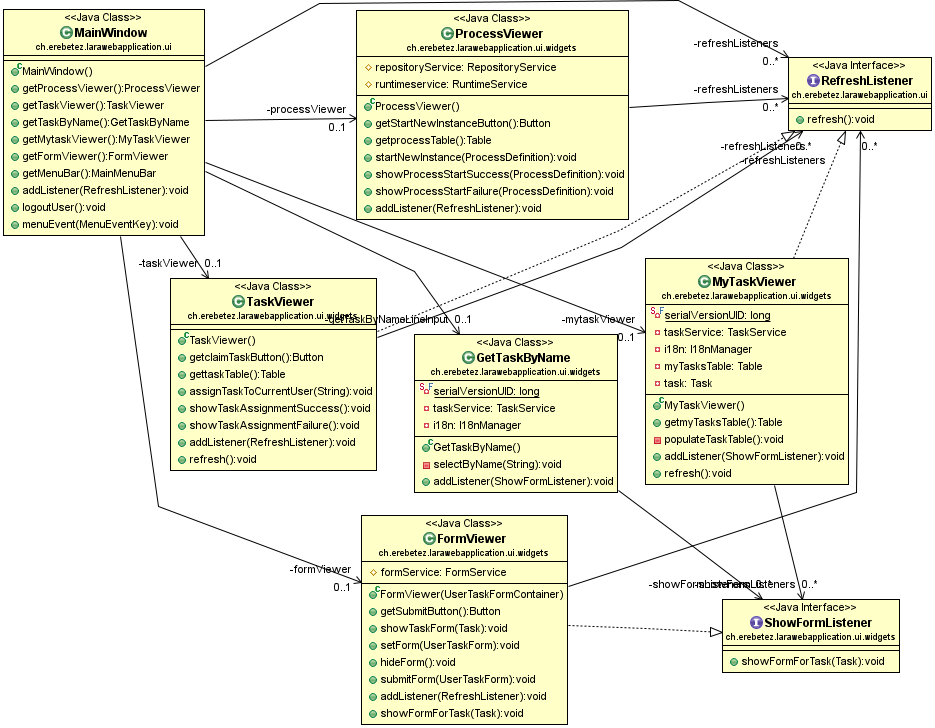
\includegraphics[width=1\textwidth]{./img/uml_webapp_model.png}\\
    \end{center}
  \caption{UML diagramm of main web application classes}
  \label{webapplicationclassuml}
\end{figure} 

The web application is a simple GUI application. As a starting point the example application "how to build a Vaadin web application on top of Activiti" was taken \cite{Vaadinactivitwebapp}, \cite{Vaadinactivitwebapp2}.

There is the main window that holds different widgets that extends from the Vaadin CustomComponent class in a layout. Each widget shows a certain
information. For example there is a process viewer that presents the available BPMN processes. 

The following widgets are implemented in the demo web application.

\begin{itemize}
 \item process viewer: shows available main processes
 \item task viewer: unassigned tasks
 \item my task viewer: shows the assigned tasks of the current user
 \item start task by id: tasks can be started by a give id
 \item form viewer: shows the form of the task that is executed
 \item history view: shows information about finished tasks and processes
\end{itemize}

There is a listener interface that can be implemented by these widgets. The task viewer listens to the process viewer if a new task is started. The
my task viewer listens to the task viewer to see if a task is being claimed. And the form viewer checks if a task is executed. When the task is
finished the task viewers are updated to show the remaining tasks.

\begin{figure}
    \begin{center}
\begin{verbatim}
@Configurable(preConstruction = true)
public class TaskViewer extends CustomComponent implements RefreshListener {

    @Autowired
    private TaskService taskService;

    ....
}
\end{verbatim}
  \caption{Example skeleton of an Vaadin CustomComponent with Activiti service}
   \end{center}
  \label{examplecodecomponent}
\end{figure} 

Since Activiti is being configured over spring, the Activiti instances can be provided as singletons to each widget that needs them. This is done with the Annotation @Autowired \cite{autowire}. This way the
process logic is being separated from the user interface.



\subsection{BPMN deployment}
The demonstration web application deploys the BPMN processes to the Activiti engine at start up. In the future and for productive use of Activiti the
BPMN process deployment should be done over a separate applications or as a function inside the web application. 
The deployment can also be done over the spring configuration.

\subsection{Internationalization}
Internationalization is only needed for the web application. Since the web application is written in basic java, the basic resource pattern can be used. That means each view able string is loaded from a resource file that holds the strings of the given local. 



\subsection{Authentication}
The user authentication can be done in the BPMN engine. The engine has to know anyway what user is currently logged in. Activiti can therefore be connected to a ldap server to retrieve the needed user login information.



\section{External application server}
The basic concept is a rpc socket client/server architecture. \cite{rpc}

\subsection{Server}
The server receives a request to execute a certain Excel application. It then executes this application. If multiple request are received they get stored in an array (queue) and then the external Excel applications are run in serial. 

\begin{figure}
    \begin{center}
       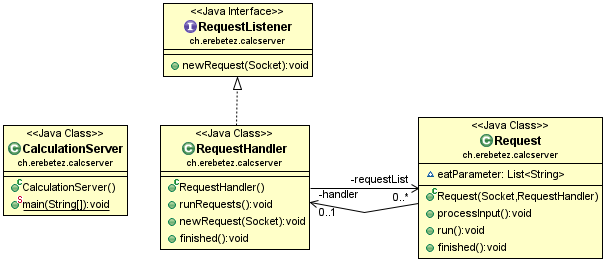
\includegraphics[width=1\textwidth]{./img/calcServerUML.png}\\
    \end{center}
  \caption{UML Class diagram of calculation server}
  \label{uml_calculationserver}
\end{figure} 


\subsection{Client}
The client is a BPMN service task for the engine server. This service task can be implemented in any process. 
The configuration of that task is made in spring. This way the methods or processes can configure their own external applications.

In the current implementations of the client service task it is possible to configure in spring the host name the port and the application name that has to be started.

The service task has to be thread save \cite{treadsave}. This is because Activiti will call the same instance of the service every time a process needs it. 

The client open a connection to the server does the communication with the defined protocol and finally writes the data back into the Activiti variable.

If an error occurs a BPMN Java exception is raised.

\begin{figure}
    \begin{center}
       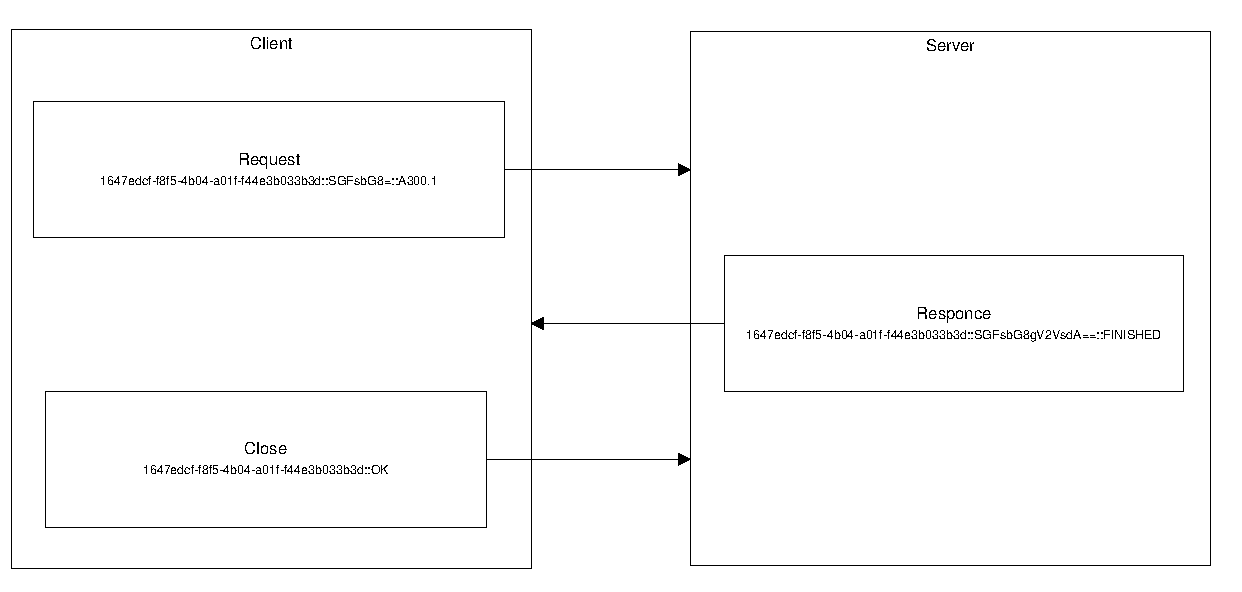
\includegraphics[width=1\textwidth]{./img/clientServerProtocoll.pdf}\\
    \end{center}
  \caption{Visualisation of client server rpc protocol}
  \label{protocol}
\end{figure} 

\subsection{Protocol}
For the communication between both parties a protocol has to be defined. 
First the client send a request to the server that has an UUID \cite{uuid}, the application to start and the marshalled data string. The marshalled data is an Java object (Nested Maps and Lists) that is converted (marshalled) in an XML string. The XML is then base64 \cite{base64} coded.
Each information is separated by two "::". The Information string send to the server then looks like that.
\begin{verbatim}
 UUID::MARSHALSTRING::APPID
 1647edcf-f8f5-4b04-a01f-f44e3b033b3d::SGFsbG8=::A300.1
\end{verbatim}

The client waits for a response. If The server cannot be reached an error is raised. 
The Activiti client task will not finish and still be in the same state as before.

The server saves the base64 coded marshall string in a file named as the UUID in a local folder.
This way the data can be used by the program the server starts (i.e here A300). 
The application safes the modified base64 marshall string back into that file as soon as the job is done.

As soon as the server has processed the request, the answer in form of the following string is send back.
The data is read from the file written by the started application.
First the UUID is given then the data as marshall string and finally the keyword "FINISHED".

\begin{verbatim}
 UUID::MARSHALSTRING::FINISHED
 1647edcf-f8f5-4b04-a01f-f44e3b033b3d::SGFsbG8gV2VsdA==::FINISHED
\end{verbatim}

The UUID has to be the same as the one the client send in the first place. If not an error is raised.

If everything is fine, the client finally sends the OK to close the connection to the server.
The finish signal looks like this.
\begin{verbatim}
 1647edcf-f8f5-4b04-a01f-f44e3b033b3d::OK
\end{verbatim}
The socket connection is then closed.

\section{Processes / Methods}
With methods analytical laboratory processes is meant. Each Method has at leas a BPML XML definition.

In addition they can have custom forms that are implemented in Java. These forms are extended from an abstract from class that knows the Activiti services. This way the forms can have the information from current execution variables or historic data from other tasks. For each form a spring bean is created in the method-context.XML file. This way it is then easy to add the form to the web application. The web application has a form container that is also configured with a spring context file.

If the process has other special service tasks the Java code can also be stored in these methods. 

All this method files are bundled in a Java jar archives and versioned separately. Unit tests can also be run over these methods.


\section{Custom Jar library's}
Jar library's are reusable packages of functions and classes. In Java the classes are put together in a jar file. These jar files can be imported in an other project and so be easily used.
Jar files can be tested separately and be provided in a maven repository.

For this project a few of these components where created. For one they would have at some point been needed anyway and for the other reason to
demonstrate the work flow with the build tools and repository.



\subsection{Data structure}
At the moment a specified data structure to store all the needed laboratory data already exists. It was implemented in vba and just consists of
arrays, dictionary's and values. These structures exists in every programming language. Therefore it is easy to port the existing structure for
example to Java. But since Java is object oriented the laboratory objects can be modelled even better than in plain old VBA. A sequence object can be
created that in turn hold assay objects that also holds result objects. Beside the basic data holding some logic can be implemented or some properties
can be extended and customized to special objects. A further benefit of having customized data objects (beans), is the fact that Vaadin provides
tables that can be filled whit Java beans.




\subsection{Marshalling}
One key feature of porting the existing Excel framework to Activiti and Java is the marshalling and unmarshalling of the data objects.
Being able to marshall an object into an XML file and sending it over a socket provides a powerful function to communicate with other programs that
might even be written in an other programming language.

The ability to marshall objects is already implemented in the existing Excel framework. So only the matching Java code has to be implemented.
With the existing XSD definition it is possible to automatically create Java objects with the xjc \cite{xjc} command line tool.
These objects can than be used with the JAXB \cite{jaxb} classes to easily navigate through the XML data and creating the Java objects.


%recursion, dict, list, values

\subsection{Compression}
\begin{figure}
    \begin{center}
      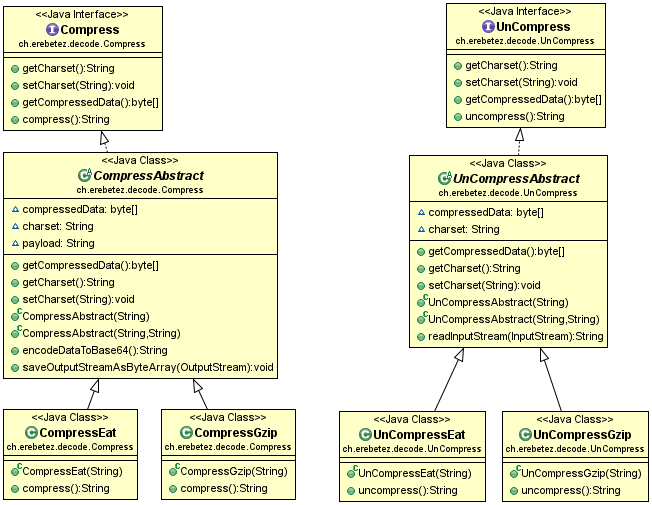
\includegraphics[width=1\textwidth]{./img/uml_decode_model.png}\\
    \end{center}
  \caption{UML class structure of the compression classes}
  \label{compressionClassUml}
\end{figure} 

Before sending the XML to another socket over the network it is usually good to compress the data.
In our case the standard inflation and deflation algorithm is used (zlib) \cite{zlib}. After the compression 
the data bytes are encoded into base64 \cite{base64}. That allows a save transmission over the TCP/IP stack.

To check that the payload was successfully send over TCP/IP the length of the uncompressed string is prepended in front of the compressed data. This way when uncompressing the string, it can be checked if both have the same length. 

The compression and the decompression classes have each an Java interface and a abstract class. This allows to implement different compression algorithms with the same basic code base. For example beside the zlib deflation zip which is used in the current Excel application a gzip compression has also been created on top of the same abstract class.


\subsection{Excel adapter}

\begin{figure}
    \begin{center}
      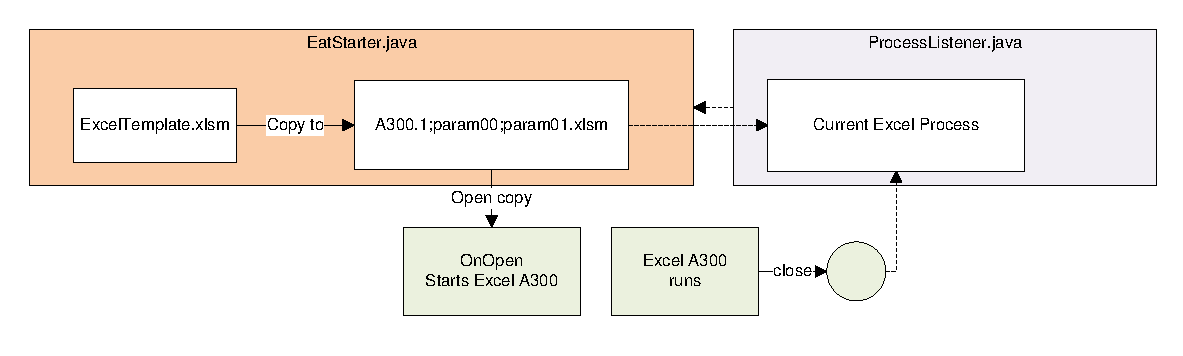
\includegraphics[width=1\textwidth]{./img/eatstarterOverview.pdf}\\
    \end{center}
  \caption{Process overview of the Excel starter}
  \label{eatstarteroverview}
\end{figure} 

In order to use the existing application stack based on Excel, it is important to be able to start Excel files from Java code. 
The Excel adapter has two parts. One is the Java package and the other is a special Excel spreadsheet. 

The Java package takes some arguments starts the Excel spreadsheet and gives a signal as soon as the Excel process has finished.

The spreadsheet to start other Excel applications has an on open method. In that method the the existing Excel applications are started with the given parameter. The trick to start Excel applications with parameter is by coping the template to a new location. The file name then represents the parameters which are separated by a separator.

A modification of the current Excel plug-in has to be made. Many functions can be removed because most logic is then done in the BPMN engine or in Java service task code.

\begin{figure}
    \begin{center}
      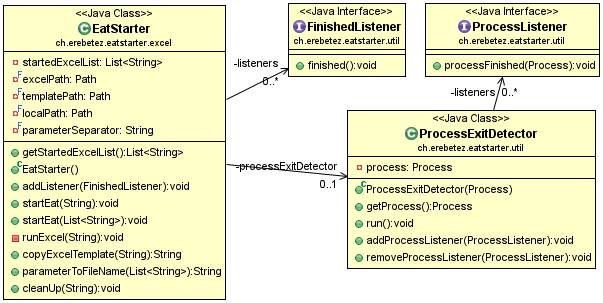
\includegraphics[width=1\textwidth]{./img/uml_eatstatreter_model.png}\\
    \end{center}
  \caption{UML class structure of the Excel starter}
  \label{eatstarterclassuml}
\end{figure} 

%TODO Excel addin




\section{Environments}
At least three environments have to be defined. Development, validation and production. 

The development environment is where the development is done. Usually the applications are run locally on the developer pc. The spring configurations can be modified at any time to match the need of the developer.
For unit testing is also done at this stage.

The validation environment should look and behave the same as the production environment. On the validation environment, the final builds are deployed. They then get tested. The formal testing is also done on the validation environment. If an error occurs during tests, a new build is created and deployed on the validation environment.

When everything looks good, a productive build based on the one from the validation environment is created and deployed on the productive environment.

Developer should also be able to pull data from the validation or productive server.

\section{Build tools}
The question what build tool, if any, came pretty early in the project development. Just starting a Project in Eclipse is the easiest way. 
At least as long as the project is not to big, is only one project and doesn't really change over time. That was all not the case. So lets have a look at few of them. 

In the Java World there are the usual suspects:
\begin{itemize}
 \item Ant
 \item Maven
 \item Gradle
\end{itemize}

\subsection{Ant}
Ant is the oldest of the three. It allows to define build scripts in XML. 
It has no own logic, so all tasks or targets have to be written from scratch.
That allows a big flexibility, it is however also quit complex. There is also the fact,
that scripting in XML is not really fun.


\subsection{Maven}
Maven also uses also XML for the configuration. Opposed to ant, you define how the project has to be build. The building is then
made by Maven. Maven also resolves dependencies. Maven is widely used and therefore has a lot of plug-ins and additional tools like an eclipse plug-in. For our case Maven seemed to do the job.


\subsection{Gradle}
Gradle is the newest member in the Java build tool family. Gradle is not just a Java build tool so i can also handle other languages. The configuration file is written in groovy. That makes a much nicer looking project definition.
Gradle also doesn't reinvent the world. It uses the same dependency resolvement as Maven. So it can almost do everything that Maven can. In addition, it is easy to create custom tasks like in ant.

The downside is, that Gradle is still a very young project and has not as much plug-ins or examples as Maven. It is however worth keeping in sight.

\subsection{Usage}
For the main web application it is the simplest way to use Maven as the build tool. Since Gradle seems very promising, the plan is to use it in the
smaller sub projects. That way it can be easily evaluated and maybe used as the main build tool in the future.


\section{Testing and Validation}
Testing and Validation is an very important subject. It begins already with the developer and goes all the way to the qc personnel.
There are several strategies to be followed.

\subsection{Unit Tests}
Unit tests are an important tool during and after the development of the code. If possible each function and each class should also have his unit test. 
Unit tests are low level tests that can be run automatically. By writing unit tests it also forces the developer to create modular and well designed classes.
The best practice is, to write the unit test first with all the requirements and then implement functionality until all tests passes. This is of course repeated task 
that goes on forever.
The big advantage of unit tests is now, that if a change in the code should brake something, at least one unit test will most likely fail.
The developer then also know where to look and fix the problem right away.

\subsection{Validation Tests}
Once the all functionality is implemented the packages and applications are build and deployed to the validation environment. The validation environment is configured as 
close as possible the same as the productive environment.

Know the testers can execute the written tests plans to check the high level functionality. This is also a formal test to conform to the regulations. If a error occurs 
the code gets modified in the development environment and redeployed. The tests are then repeated where needed.

If for example a component gets updated, the application that uses it has to be rebuild. Because the components can be tested very good with unit tests, the should already work correctly when deployed to the validation environment.
The new package does then not have to be fully tested.

\section{Versioning}
For the versioning of the source code there are several products available. Just to name a few of them: SVN, mercurial, git.
During the development of the example git was used. It is has a decentralised architecture. So every developer has always the full power of git at his disposal. It is also easy to create branches and to create labels for realises.

\begin{figure}
    \begin{center}
       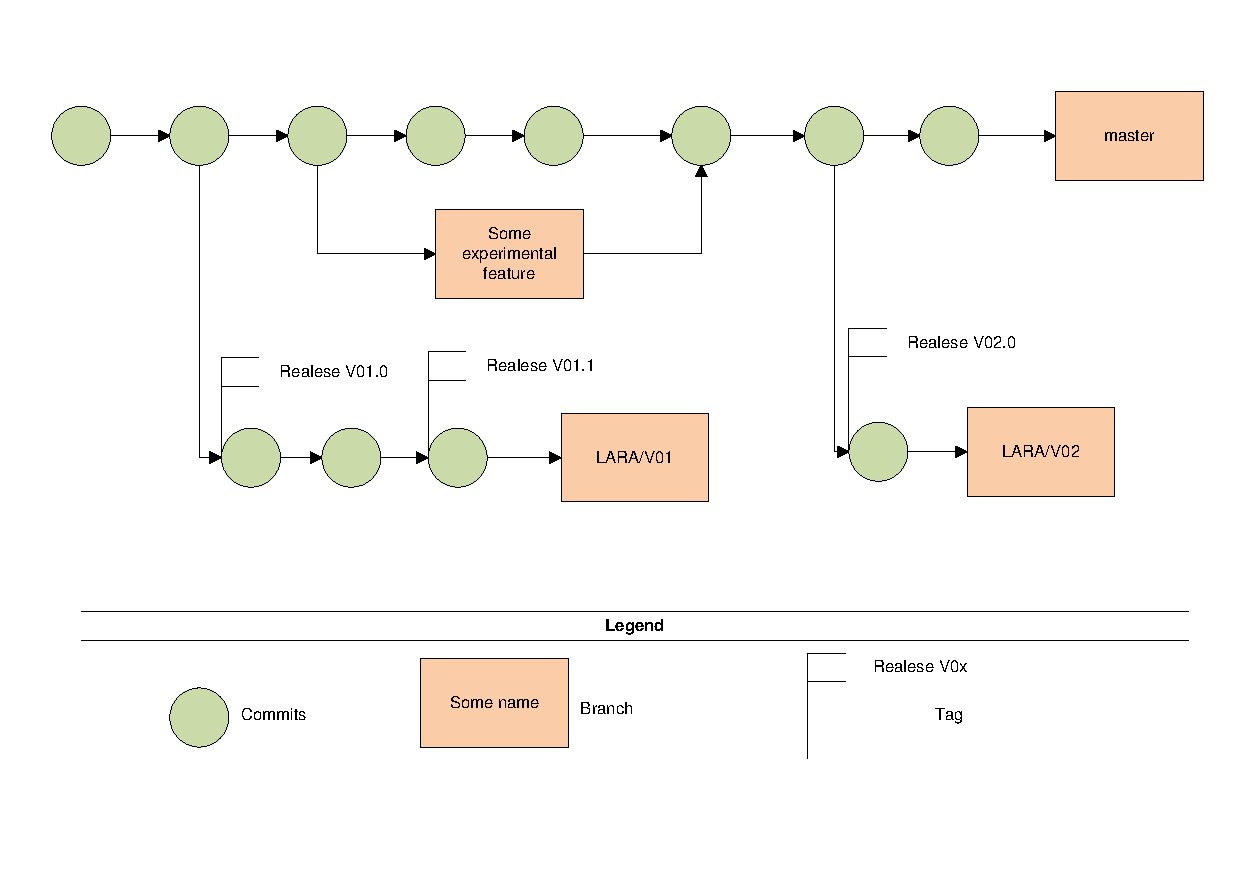
\includegraphics[width=0.9\textwidth]{./img/gitversioning.pdf}\\
    \end{center}
  \caption{Concept of the git branches}
  \label{gitbranchconcept}
\end{figure} 

\subsection{using git}
In order that every user uses the branches the same way, a few ground rules have to be set.
Each git repository will have at least three branches. productive, validation, and master.

Master is always the newest development branch. When the new feature is ready the changes are merged into the validation branch where they are tested. This validation branch gets the name of the new version.
The only thing that has to be changed in the application configuration, is the database configuration in the spring context files.
The same has to be done when the productive package is about to be build. Since the configuration for the validation and productive 
environment can be in a separate file, the change is minimal. Only some imports in the spring context XML have to be changed.

Multiple git repository will be created. The following projects shall have a own repository.
\begin{itemize}
 \item Web application
 \item External calculation Server
 \item The components
\end{itemize}

This way it is easier to manage branches and versions of each application.



\section{Deployment}
The deployment should be automated as much as possible to provide a consistent and reproducible build.
Where possible the build scripts like Maven or Gradle should be used. 
In addition to them specific shell scripts can be created.

For the web application the following steps will be required.
\begin{itemize}
 \item pack the war archive
 \item copy war archive to web application server
 \item update the BPMN process definition
\end{itemize}

The BPMN process definition a bit trickier. The XML resides in the methods jar archives. So they are in the war package. It is however needed to register them in the BPMN engine. 
This can be done with an extra program over an administration user interface. After the upload to the BPMN engine database the XML is stored in the database.

Processes started with the old process definition will finish with the definition they where started.



\subsection{Maven repository}
As Maven repository the product nexus \cite{nexus} from Sonatype is used. It is written in Java an can be deployed everywhere. I provides a nice web application to manage the repositories. The web application runs on an simple jetty \cite{jetty} application server.

Maven distinguishes two versions packages types snapshot and releases.
During the development the version is suffixed by SNAPSHOT (i.e. 1.3.1-SNAPSHOT).
This has the effect that, if such a package is put in the dependencies of an project, Maven will get the newest version of this SNAPSHOT. To force the update use -U as a parameter for Maven.
\begin{verbatim}
 mvn -U clean package
\end{verbatim}

If the package is finally tested the SNAPSHOT suffix gets removed and the package gets uploaded to the releases repository. In this repository the version can only be uploaded once. The next time a new version number has to be created.

\section{Infrastructure}
This chapter shall give an overview how the infrastructure that supports the web application and the development of it, has to look. 
All named server are planed to be virtual machines.

\begin{figure}
    \begin{center}
       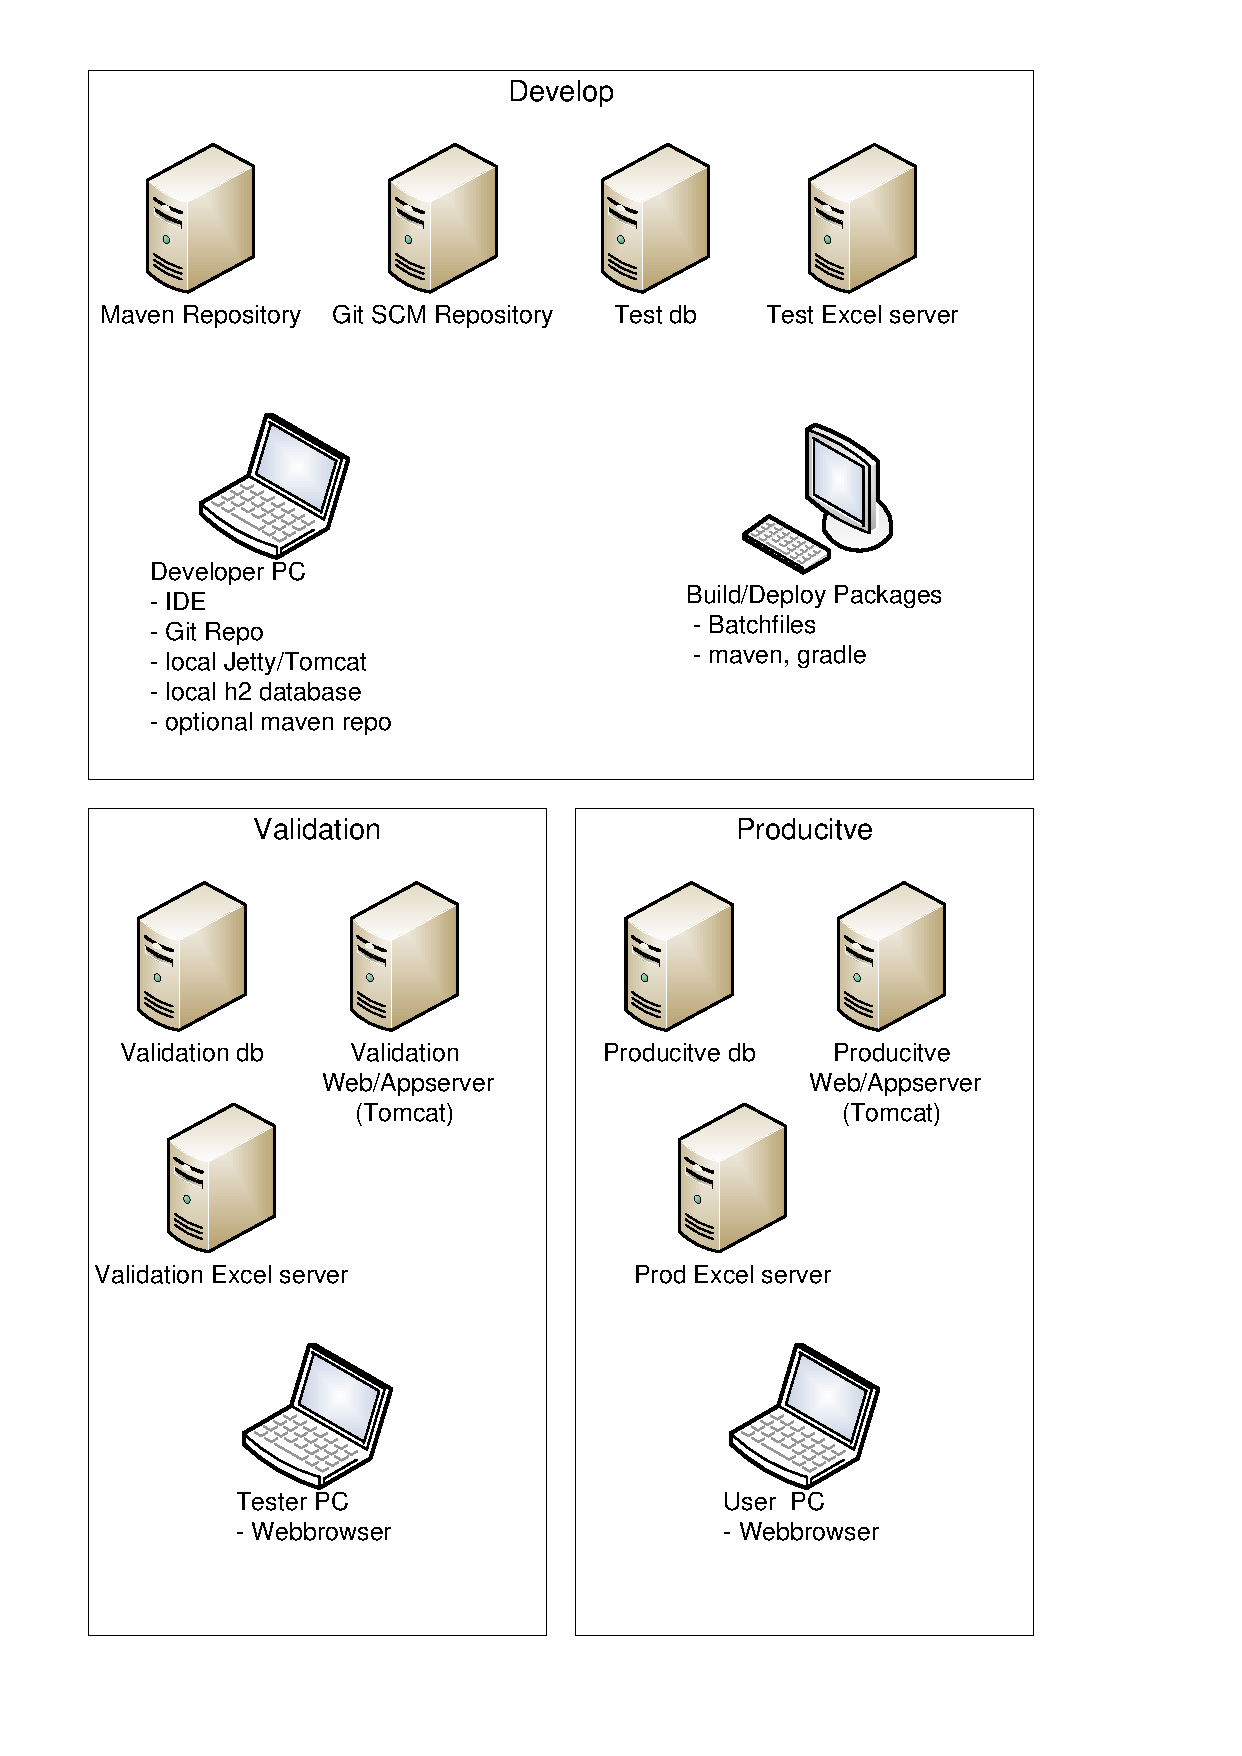
\includegraphics[width=0.8\textwidth]{./img/InfrastructureLayout.pdf}\\
    \end{center}
  \caption{Infrastructure overview}
  \label{infrastructureoverview}
\end{figure} 

It would have four servers. 
\begin{itemize}
 \item Web application server
 \item Database server
 \item Calculation server (Excel, r)
 \item Repository server
\end{itemize}

\subsection{Web application server}
This server is a classic web application server that can run war Archives. 
So it runs an Jee environment like jBoss \cite{jboss} or tomcat \cite{tomcat}.
The operating system is therefore not so relevant. 

To keep things simple Linux was chosen for the example server. A Windows server would work just as well.

%\subsubsection{configuration}
%configs....


\subsection{Database server}
De database server would be used to store the Activiti data. The databases supported by Activiti are mysql \cite{mysql}, oracle \cite{oracledb}. MSsql \cite{mssql} is jet in experimental state.
 
For the example a Linux server with a mysql database was setup.
To manage the database phpmyadmin \cite{phpmyadmin} is used.

Since the database is configured in the web application with spring, it is very easy to change the used database.


\subsection{Calculation server}
This is a rather exotic configuration. This server should be able to run Excel. Therefore windows is the only option al the operating system. On this server there will also run the calculation server (Java) which listens to the query of an Activiti task.



\subsection{Repository server}
This server would not be used in the productive setting. It is just there to facilitate the developers work.
The server would provide a Maven repository and a git repository. 

The operating system would be preferably Linux. That is because git is native to Linux.
For the Maven repository nexus from Sonatype would be a nice choice. It supports all neccesery functions and provides a nice web front-end for managing the repositories.

% see chapter? configuration....




\section{Conclusion}
First it is relay worth to look around and see what solutions are already available. The BPMN 2.0 standard and the engines that cat run it is a fine 
idea and very precious for any type of business. It has a big advantage of being able to design the business process and at the same time having an easy way to make it automated in a system.
At this point it must been said, that the implementations still requires specialised employees that should also be able to read some XML. The BPMN engine should also not being misused for low level tasks. At some point it is smarter to make the easy logic in an service task instead of creating yet another BPMN sup process.




\subsection{Future}
Once the process engine is in place, the functionality that is currently implemented in Excel can be migrated step by step to Java service tasks or script tasks. The goal is that finally only some calculation have to be made in Excel.

To handle the processes packages and the releases of the different software some additional administration tools have to be created. This can be an web application or just a shell script.


\newpage

\addcontentsline{toc}{section}{Bibliography}
\begin{thebibliography}{99}

\bibitem{lims} \url{http://en.wikipedia.org/wiki/Laboratory_information_management_system}

\bibitem{sdms} \url{}

\bibitem{gmp} \url{http://en.wikipedia.org/wiki/Good_manufacturing_practice}

\bibitem{eln} \url{http://en.wikipedia.org/wiki/Electronic_lab_notebook}

\bibitem{excel} \url{http://office.microsoft.com/en-us/excel}

\bibitem{bpel} \url{http://en.wikipedia.org/wiki/Business_Process_Execution_Language}

\bibitem{bpmn} \url{http://www.bpmn.org/}

\bibitem{soa} \url{http://en.wikipedia.org/wiki/Service-oriented_architecture}

\bibitem{middleware} \url{http://en.wikipedia.org/wiki/Middleware}

\bibitem{omg} \url{http://www.omg.org/}

\bibitem{activiti} \url{http://www.activiti.org/}

\bibitem{css} \url{http://en.wikipedia.org/wiki/Cascading_Style_Sheets}

\bibitem{activitijavadoc} \url{http://activiti.org/javadocs/index.html}

\bibitem{jbpm} \url{https://www.jboss.org/jbpm/}

\bibitem{activevos} \url{http://www.activevos.com/}

\bibitem{activvosscost} \url{http://www.activevos.com/content/blog/activevos2009butlergrouptechnicalaudit.pdf}

\bibitem{appacheODE} \url{https://ode.apache.org/}

\bibitem{aris} \url{https://www.softwareag.com/ch/products/wm/bpm/default.asp}

\bibitem{ariscost} \url{http://gothamschools.org/2010/09/15/frustrated-with-citys-data-system-teachers-build-their-own/}

\bibitem{biztalk} \url{http://www.microsoft.com/biztalk}

\bibitem{biztalkcost} \url{http://www.microsoft.com/biztalk/en/us/pricing-licensing.aspx}

\bibitem{signavio} \url{http://www.signavio.com/en.html}

\bibitem{eclipse} \url{http://www.eclipse.org} %FIXME

\bibitem{rpc} \url{http://en.wikipedia.org/wiki/Remote_Procedure_Call}

\bibitem{treadsave} \url{http://en.wikipedia.org/wiki/Thread_safety}

\bibitem{uuid} \url{http://en.wikipedia.org/wiki/Universally_unique_identifier}

\bibitem{Vaadin} \url{http://www.Vaadin.com}

\bibitem{gwt} \url{https://developers.google.com/web-toolkit/}

\bibitem{Vaadinactivitwebapp} \url{https://Vaadin.com/wiki/-/wiki/Main/Building Vaadin Applications on top of Activiti}

\bibitem{Vaadinactivitwebapp2} \url{https://github.com/peholmst/ActivitiVaadinDevoxx11}

\bibitem{ant} \url{https://ant.apache.org/}

\bibitem{maven} \url{https://maven.apache.org/}

\bibitem{gradle} \url{http://www.gradle.org/}

\bibitem{spring} \url{http://www.springsource.org/}

\bibitem{dependencyInection} \url{http://en.wikipedia.org/wiki/Dependency_injection}

\bibitem{autowire} \url{https://Vaadin.com/wiki/-/wiki/Main/Spring+Integration}

\bibitem{mysql} \url{https://www.mysql.com/}

\bibitem{phpmyadmin} \url{http://www.phpmyadmin.net/home_page/index.php}

\bibitem{oracledb} \url{http://www.oracle.com/de/products/database/index.html}

\bibitem{mssql} \url{http://www.microsoft.com/sqlserver/en/us/default.aspx}

\bibitem{nexus} \url{http://www.sonatype.org/nexus/}

\bibitem{jetty} \url{http://jetty.codehaus.org/jetty/}

\bibitem{jboss} \url{http://www.jboss.org/}

\bibitem{tomcat} \url{http://tomcat.apache.org/}

\bibitem{git} \url{http://git-scm.com/}

\bibitem{zlib} \url{http://zlib.net/}

\bibitem{base64} \url{http://en.wikipedia.org/wiki/Base64}

\bibitem{xjc} \url{http://docs.oracle.com/javase/6/docs/technotes/tools/share/xjc.html}

\bibitem{jaxb} \url{http://www.oracle.com/technetwork/articles/javase/index-140168.html}

\end{thebibliography}

\end{document}

